\chapter{Giải Hệ Phương Trình Và Phân Tích Hiệu Năng}

\newpage

\section{Cơ sở lý thuyết}
Phân tích hiệu năng của các thuật toán giải hệ $Ax = b$ được xây dựng trên sự tương tác giữa đặc tính cấu trúc của ma trận và triết lý tính toán của thuật toán.

\begin{itemize}[topsep=0pt, itemsep=2.5pt, leftmargin=1.5cm]
    \item Ma trận Đối xứng Xác định Dương (SPD): Sở hữu phổ trị riêng thực dương ($\lambda_i > 0$). Các hệ SPD thực tế thường được khống chế tốt (well-conditioned), đóng vai trò như một "bộ giảm xóc số học", phong tỏa sự khuếch đại nhiễu và đảm bảo sự hội tụ cho phương pháp lặp.
    \item Ma trận Hilbert: Nguyên mẫu kinh điển của sự suy biến cực đoan (ill-conditioned). Dù mang cấu trúc SPD, các trị riêng của nó phân rã về $0$ theo hàm mũ, khiến định thức tiệm cận $0$.
    \item Số điều kiện ($\kappa(A)$): Thước đo độ nhạy hệ thống (với SPD, $\kappa = \lambda_{max}/\lambda_{min}$). Theo định lý nhiễu loạn, sai số nghiệm tỷ lệ thuận với $\kappa$. Trên hệ Hilbert, $\kappa$ bùng nổ vượt quá giới hạn biểu diễn của số thực 64-bit, trở thành thứ phá hủy mọi nỗ lực tính toán.
\end{itemize}

Các bộ giải được chia thành hai trường phái, đối mặt với sự suy biến theo những cách khác biệt:

\begin{itemize}[topsep=0pt, itemsep=2.5pt, leftmargin=1.5cm]
    \item Nhóm Phương pháp Trực tiếp (Direct Methods)
    Đặc trưng bởi tính tất định, giải bài toán trong số bước $\mathcal{O}(N^3)$ hữu hạn, nhưng phải chịu "thuế tích lũy sai số cơ học":
    \begin{itemize}[label=\ding{111}, leftmargin=1.5cm]
        \item Khử Gauss ($A=LU$): Tối ưu hóa tốc độ phần cứng cực tốt nhưng sử dụng các biến đổi không trực giao. Rất dễ bị phá hủy bởi hiện tượng sụp đổ phần tử trục (pivot collapse) và khuếch đại nhiễu trên ma trận xấu.
        \item Phân rã SVD ($A=U\Sigma V^T$): Tiêu chuẩn vàng về độ ổn định ngược. Các phép biến đổi trực giao đẳng cự ($\kappa=1$) giúp SVD không bao giờ tự sinh/khuếch đại rác số học. Điểm yếu là chi phí tính toán siêu việt khổng lồ và dễ mất toàn bộ tính ổn định nếu lập trình ngây thơ qua bước nhân hiệp phương sai $A^T A$.
    \end{itemize}
    \item Phương pháp Lặp (Iterative Methods): Gauss-Seidel: Khả năng hội tụ bị quyết định tuyệt đối bởi bán kính phổ của ma trận lặp ($\rho < 1$). Trên hệ SPD lý tưởng, thuật toán tạo ra cơ chế nén sai số chủ động. Tuy nhiên, trên hệ suy biến như Hilbert, do $\rho \to 1$, động năng tiệm cận bị triệt tiêu hoàn toàn, ép hệ thống rơi vào trạng thái đình trệ giải tích (stagnation) vĩnh viễn.
\end{itemize}

\section{Phân tích hiệu năng}
Qua quá trình đối chiếu thực nghiệm trên hai hệ không gian đối lập (SPD khống chế tốt và Hilbert khống chế cực kém), hiệu năng của ba bộ giải tuyến tính bộc lộ rõ bản chất đánh đổi tàn khốc của Giải tích số:

\begin{figure}[h!]
    \centering
    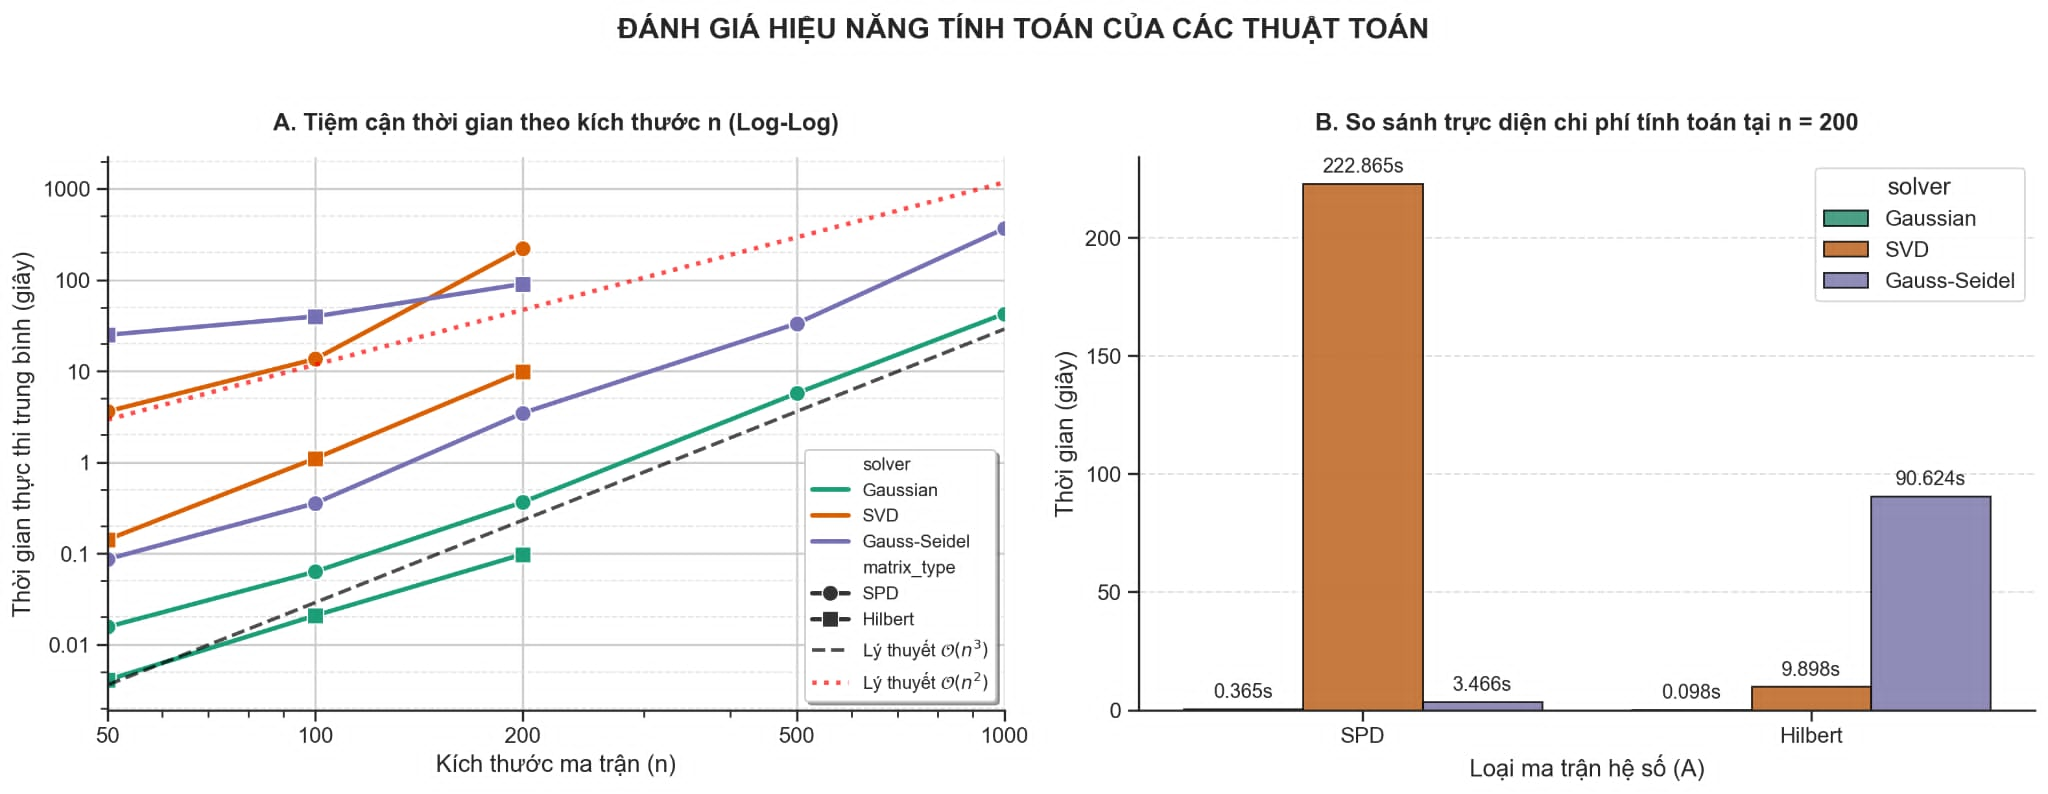
\includegraphics[width=1.0\textwidth]{images/chapter_03/time-execute.png}
    \caption{Thời gian thực thi}
    \label{fig:niuq}
\end{figure}

\begin{itemize}[topsep=0pt, itemsep=2.5pt, leftmargin=1.5cm]
    \item Khử Gauss (Đỉnh cao Tốc độ & Vực thẳm Suy biến): Đại diện cho sự tối ưu hóa vi kiến trúc cực đại với các lệnh FMA (nhân-cộng), cho thời gian thực thi nhanh nhất. Tuy nhiên, phép biến đổi không trực giao khiến nó trở thành nạn nhân của sự bào mòn sai số cơ học $\mathcal{O}(N^3)$. Trên không gian suy biến (Hilbert), sự sụp đổ của phần tử trục tạo ra Thảm họa Bùng nổ Sai số, phá hủy hoàn toàn cả phần dư lẫn vector nghiệm.
    \item SVD (Hàng rào Hình học & Lỗ hổng Triển khai): Được thiết kế như một tấm khiên tuyệt đối chống lại nhiễu nội sinh nhờ các phép quay trực giao đẳng cự. Tuy nhiên, phương pháp này chịu hình phạt khổng lồ về thời gian chạy do độ phức tạp của hàm siêu việt. Nghiêm trọng hơn, thực nghiệm chứng minh SVD rất mong manh trước lỗi cài đặt: Việc khởi tạo gián tiếp qua hiệp phương sai $A^T A$ đã châm ngòi cho hiện tượng Tràn số dưới (Underflow), dẫn đến Thất bại Tĩnh lặng (Hội tụ giả) trên hệ Hilbert và đánh mất hoàn toàn lợi thế chính xác lý tưởng.
    \item Gauss-Seidel (Kiểm soát Chủ động & Đình trệ Phổ): Đại diện cho triết lý hậu kiểm mục tiêu. Trên hệ ổn định (SPD), việc sử dụng chuẩn $L_2$ giúp thuật toán tạo ra Hiệu ứng Nén Sai số, ép buộc các biến số phải chính xác hơn khi không gian mở rộng (đánh đổi bằng chi phí lặp). Dẫu vậy, khi đối mặt với hệ suy biến ($\rho \to 1$), động năng hội tụ bị triệt tiêu, ép hệ thống vào trạng thái Đình trệ Giải tích. Sự đình trệ này, kết hợp với hiệu ứng bình phương nhiễu trắng của chuẩn $L_2$, vô tình đánh lừa các tiêu chuẩn dừng, khiến thuật toán nghiệm thu các "nghiệm rác" mà không hề hay biết.
\end{itemize}

Thực nghiệm khẳng định một tiên đề tối thượng trong Khoa học máy tính: Không tồn tại một thuật toán hoàn hảo cho mọi không gian dữ liệu. Trong khi Phương pháp Trực tiếp bị giới hạn bởi sự tích lũy nhiễu cơ học $\mathcal{O}(N^3)$, thì Phương pháp Lặp bị trói buộc bởi động năng của Bán kính phổ. Hơn thế nữa, dù thuật toán có thiết lập hàng rào phòng thủ vững chắc đến đâu (như SVD), giải tích số vĩnh viễn không thể vượt qua ranh giới vật lý áp đặt bởi Số điều kiện $\kappa(A)$ của ma trận. Lựa chọn bộ giải là nghệ thuật đánh đổi giữa Tốc độ Vi kiến trúc, Độ ổn định Hình học và Sự thấu hiểu sâu sắc về Độ nhạy Hệ thống.

\section{Phân tích độ ổn định}

\subsection{Hệ ma trận SPD (well-conditioned)}

Nhằm làm rõ bản chất thực sự của các bộ giải tuyến tính, phần dưới đây sẽ đi sâu phân tích biểu đồ quỹ đạo sai số trên không gian ma trận khống chế tốt (SPD). Việc đặt các thuật toán vào một môi trường dữ liệu hoàn hảo sẽ bóc trần một nghịch lý thú vị của Giải tích số: phương pháp được thiết kế với rào chắn an toàn cao nhất lại không phải là phương pháp chạm đến đáy sai số của máy tính

\begin{figure}[h!]
    \centering
    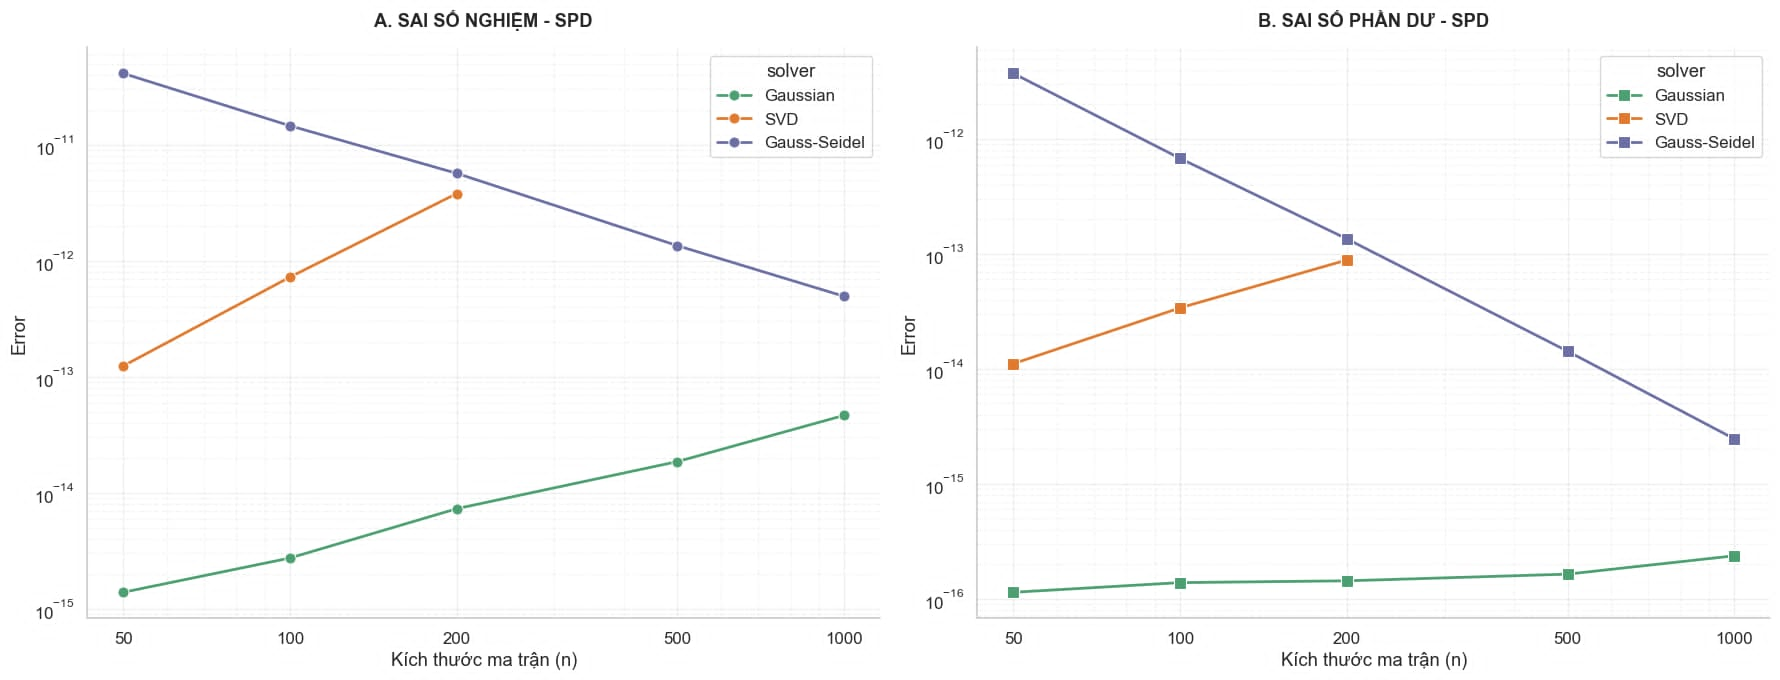
\includegraphics[width=1.0\textwidth]{images/chapter_03/spd.png} % <- path tới cái image / xóa dấu .. trong path đi
    \caption{Sai số trên hệ SPD} % <- caption là gì m / dòng chữ dưới tấm hình
    \label{fig:niuq} % vậy label là gì / này t ko bt, xóa cũng đc
\end{figure}

\begin{itemize}[topsep=0pt, itemsep=2.5pt, leftmargin=1.5cm]
    \item Khử Gauss (Tối ưu Vi kiến trúc & Chạm đáy Phần cứng): Được bảo chứng độ an toàn tuyệt đối bởi cấu trúc SPD (không xảy ra sụp đổ phần tử trục), thuật toán tận dụng tối đa tốc độ của tập lệnh nhân-cộng cơ sở (FMA) để vắt kiệt năng lực tính toán của Float64, đưa vector nghiệm cắm thẳng xuống và neo chặt tại giới hạn sai số tận cùng của máy tính (Machine Epsilon $\approx 10^{-16}$).
    \item SVD (Thuế Lượng giác & Suy hao Biến đổi): Mặc dù được bảo vệ bởi phép quay trực giao lý tưởng, thuật toán vẫn phải chịu mức sai số cao hơn Khử Gauss do gánh chịu "thuế tích lũy cơ học" sinh ra từ $\mathcal{O}(N^3)$ phép tính hàm siêu việt (lượng giác), cộng hưởng với lượng thông tin bị suy hao ngay từ bước nhân ma trận hiệp phương sai $A^T A$ sơ khởi.
    \item Gauss-Seidel (Kiểm soát Chủ động & Giới hạn Tiêu chuẩn): Thể hiện triết lý tối ưu thực dụng khi lơ lửng ở mức sai số cao nhất trên đồ thị không phải do bất ổn, mà do cơ chế hậu kiểm $L_2$ đã chủ động dừng thuật toán ngay khi vừa chạm ngưỡng dung sai (tolerance) do con người áp đặt, thành công trong việc tiết kiệm tài nguyên lặp và từ chối việc chạy đua độ chính xác dư thừa.
\end{itemize}

Trên một không gian dữ liệu lý tưởng như SPD, các giới hạn toán học lùi lại phía sau, nhường chỗ cho ranh giới của phần cứng và triết lý lập trình. Khử Gauss vươn tới giới hạn tuyệt đối của máy móc, SVD chịu thuế nhiễu loạn của khối lượng tính toán, trong khi Gauss-Seidel dừng lại ở giới hạn của nhu cầu thực tiễn.

\subsection{Hệ ma trận Hillbert (ill-conditioned)}

\subsubsection{Phương pháp Trực tiếp (Direct Methods)}

Nhóm phương pháp trực tiếp, đại diện tiêu biểu bởi thuật toán Khử Gauss và Phân rã giá trị suy biến (SVD), được xây dựng trên triết lý giải tích tất định: cam kết tìm ra nghiệm chính xác thông qua một chuỗi hữu hạn các phép phân rã cấu trúc ma trận. Phần dưới đây sẽ đi sâu phân tích cơ chế hoạt động của nhóm thuật toán này, làm rõ sự đánh đổi khốc liệt giữa lợi thế tối ưu hóa vi kiến trúc phần cứng và rủi ro tàn khốc của việc tích lũy sai số cơ học $\mathcal{O}(N^3)$ khi không gian tính toán mở rộng

\begin{figure}[h!]
    \centering
    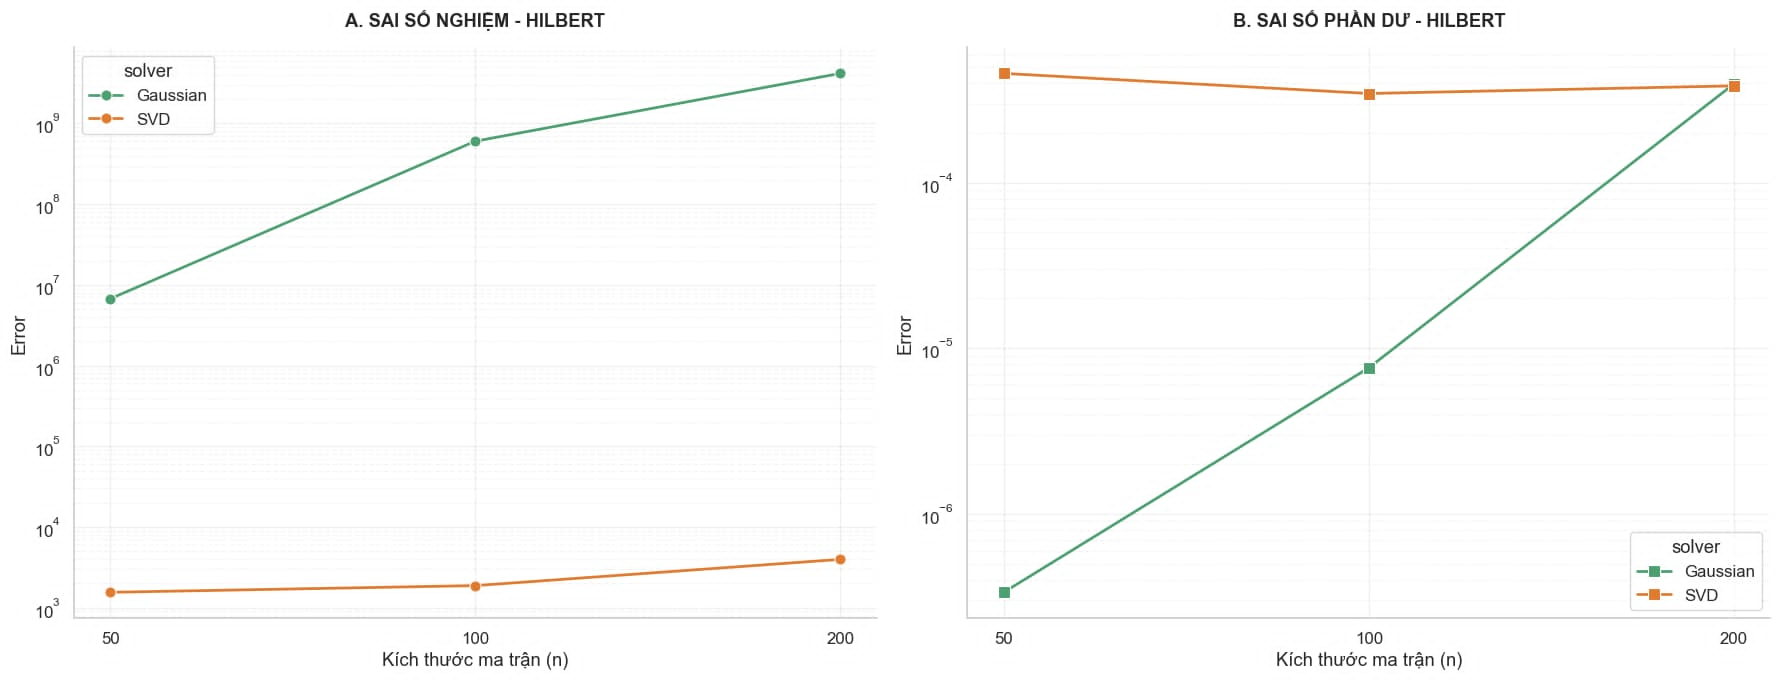
\includegraphics[width=1.0\textwidth]{images/chapter_03/hillbert.png} % <- path tới cái image / xóa dấu .. trong path đi
    \caption{Sai số trên hệ Hillbert} % <- caption là gì m / dòng chữ dưới tấm hình
    \label{fig:niuq} % vậy label là gì / này t ko bt, xóa cũng đc
\end{figure}

\begin{itemize}[topsep=0pt, itemsep=2.5pt, leftmargin=1.5cm]
    \item Khử Gauss (Đỉnh cao Vi kiến trúc & Vực thẳm Số học): Trên hệ SPD, Khử Gauss thống trị tuyệt đối về tốc độ nhờ tối ưu hóa lệnh FMA, vắt kiệt năng lực phần cứng để chạm đáy sai số Machine Epsilon ($10^{-16}$). Tuy nhiên, phép biến đổi không trực giao khiến nó sụp đổ tàn khốc trên hệ Hilbert: sự sụp đổ của phần tử trục tạo ra lượng rác số học khổng lồ, bùng nổ phi mã qua hệ số khuếch đại $\kappa$, phá hủy hoàn toàn cả vector nghiệm lẫn phần dư.
    \item SVD (Ảo ảnh Trực giao & Lỗ hổng Triển khai): SVD dùng phép quay trực giao ($\kappa=1$) để khóa chặt rác nội sinh, duy trì sự ổn định lý thuyết. Tuy nhiên, nó phải trả "thuế độ phức tạp" khổng lồ cho các phép toán lượng giác. Trầm trọng hơn, việc triển khai SVD gián tiếp qua $A^T A$ đã tự triệt tiêu thông tin ma trận, gây tràn số dưới (underflow) trên hệ Hilbert, dẫn đến "Thất bại tĩnh lặng" (hội tụ giả) thay vì một sự bảo vệ hình học như lý thuyết hứa hẹn.
\end{itemize}

\subsubsection{Phương pháp Lặp (Iterative Methods)}

Gauss-Seidel (Cơ chế Nén Chủ động & Bẫy Đình trệ Giải tích):

Trên hệ SPD, tiêu chuẩn chuẩn $L_2$ tạo ra "Hiệu ứng nén sai số", ép buộc hệ thống tự động thắt chặt độ chính xác của từng biến số cho đến khi lọt qua ngưỡng dung sai (tolerance) do con người áp đặt. Tuy nhiên, phương pháp lặp hoàn toàn bất lực trước sự biến dạng không gian. Trên hệ Hilbert, khi bán kính phổ tiệm cận 1 ($\rho \to 1$), động năng hội tụ bị triệt tiêu. Hệ thống rơi vào "Đình trệ giải tích", kết hợp với hiệu ứng underflow của việc bình phương chuẩn $L_2$, vô tình đánh lừa thuật toán nghiệm thu một vector rác trong sự cạn kiệt của tài nguyên thời gian (max_iter).

\section{Kết luận}
Thông qua việc đối chiếu hành vi của các bộ giải trên hai hệ không gian đối lập, thực nghiệm đã chứng minh một chân lý cốt lõi của Giải tích số: Độ ổn định của một nghiệm cuối cùng không được quyết định bởi sự ưu việt của thuật toán, mà bị chi phối tuyệt đối bởi bản chất của không gian ma trận. Sự phân hóa này được thể hiện qua hai thái cực:

\begin{itemize}[topsep=0pt, itemsep=2.5pt, leftmargin=1.5cm]
    \item Ma trận SPD (Vùng an toàn của Vi kiến trúc): Với đặc tính đối xứng và được khống chế tốt (số điều kiện $\kappa$ nhỏ), hệ SPD hoạt động như một "bộ giảm xóc số học" hoàn hảo. Nó phong tỏa sự khuếch đại sai số, cho phép các thuật toán bộc lộ tối đa năng lực lý thuyết của mình. Tại đây, Khử Gauss vươn tới giới hạn tột cùng của phần cứng (Machine Epsilon), SVD duy trì sự ổn định trực giao, và Gauss-Seidel hội tụ an toàn về đúng ngưỡng dung sai mục tiêu. Trên không gian này, rào cản duy nhất là giới hạn vật lý của máy tính và nhu cầu của con người.
    \item Ma trận Hilbert (Bản án của Sự suy biến):Trái ngược hoàn toàn, hệ Hilbert đại diện cho sự bóp méo thông tin cực đoan. Số điều kiện khổng lồ ($\kappa \approx 10^{19}$) trở thành một lăng kính khuếch đại tàn nhẫn, biến những nhiễu loạn cơ học vi mô thành thảm họa vĩ mô. Tại đây, mọi lưới bảo vệ của thuật toán đều bị xé toạc: Khử Gauss chết vì bùng nổ rác nội sinh, SVD chết vì tràn số dưới, và Gauss-Seidel chết vì đình trệ động năng. Không một kỹ thuật tối ưu mã nguồn nào có thể cứu vãn được hệ thống.
\end{itemize}
